% Provenance (never printed): cycle 3 / 6e "La planete Terre, l'environnement
% et l'action humaine" (the Earth in the Solar System; conditions for life);
% see sources/book1/PROVENANCE.md. Book 1, grade 6, chapter 1.
\chapter{La Terre, une planète du Système solaire}\label{ch:g6:earth-a-planet}

Trois sondes robotisées ont été envoyées dans l'espace. L'une après
l'autre, elles envoient une image vers la Terre, comme une carte postale.
La première vient de Vénus~: une boule pâle enveloppée d'épais \omterm{def:g4:clouds-rain-snow:cloud}{nuages}, où
il fait assez chaud pour faire fondre le plomb et où l'air presse sur le
sol d'un poids écrasant. La deuxième vient de Mars~: un \omterm{def:g5:weather-and-climate:desert}{désert} rouge, froid
et poussiéreux, sous un ciel ténu. La troisième sonde a tourné sa caméra
vers chez nous~: une boule bleue et blanche, avec des \omterm{def:g2:water-on-earth:ocean}{océans}, des \omterm{def:g4:clouds-rain-snow:cloud}{nuages} et
de la glace. Trois planètes, voisines autour du même Soleil. Pourquoi une
seule d'entre elles est-elle bleue~?
% ledger: nasa:venus-clouds, nasa:mars-water

\begin{omfigure}
\begin{minipage}[t]{0.31\linewidth}\centering
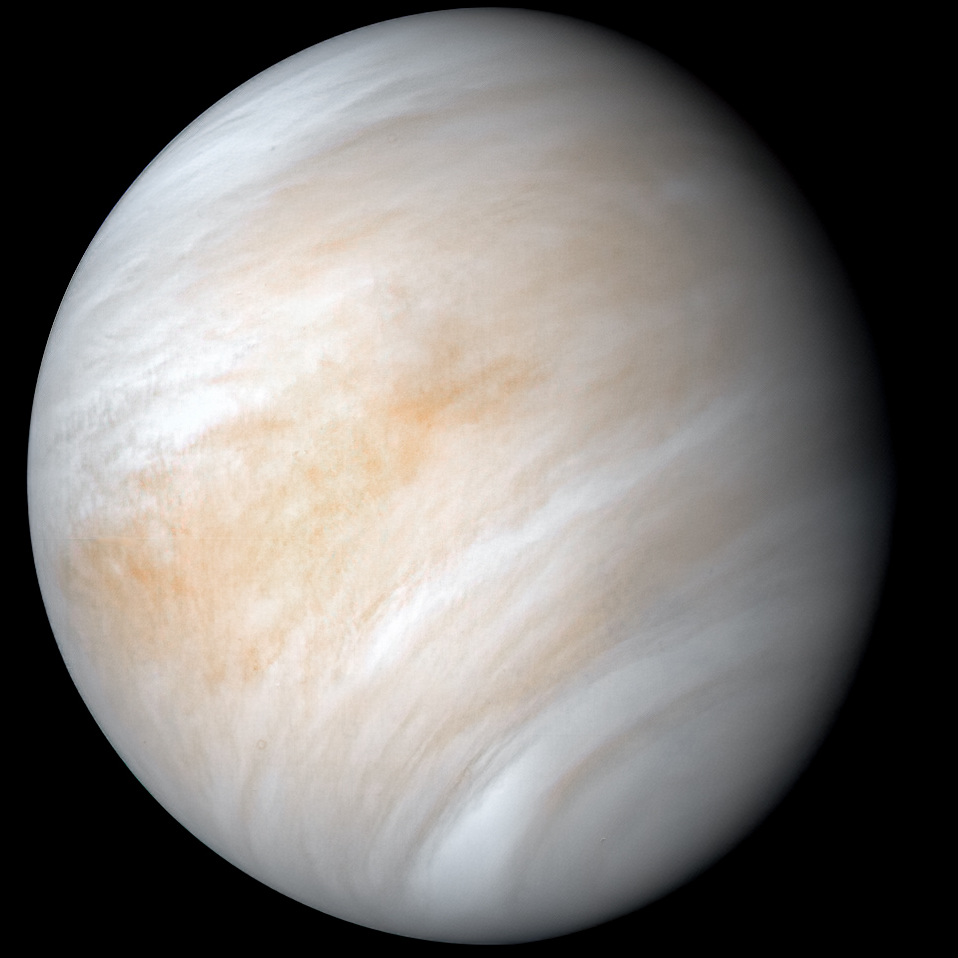
\includegraphics[width=\linewidth]{images/book1/g6-venus-mariner10.jpg}\\[2pt]
{\small Vénus}
\end{minipage}\hfill
\begin{minipage}[t]{0.31\linewidth}\centering
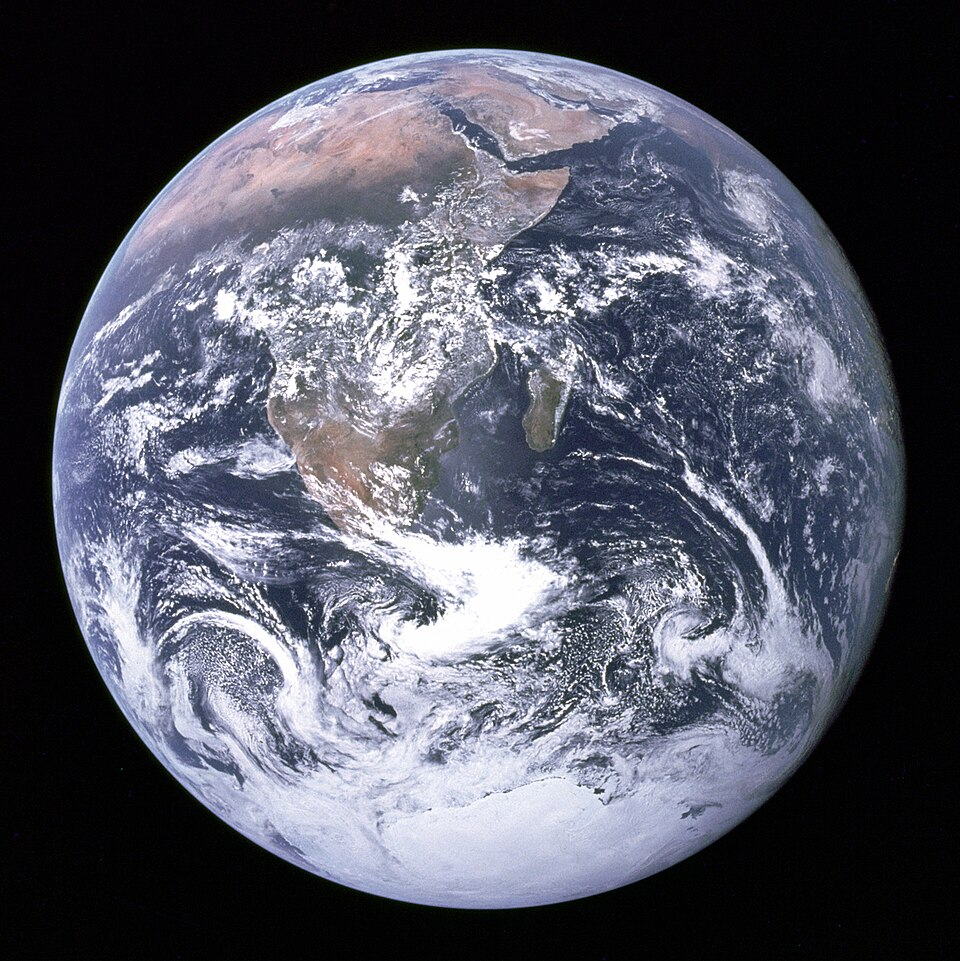
\includegraphics[width=\linewidth]{images/book1/g6-earth-apollo17.jpg}\\[2pt]
{\small La Terre}
\end{minipage}\hfill
\begin{minipage}[t]{0.31\linewidth}\centering
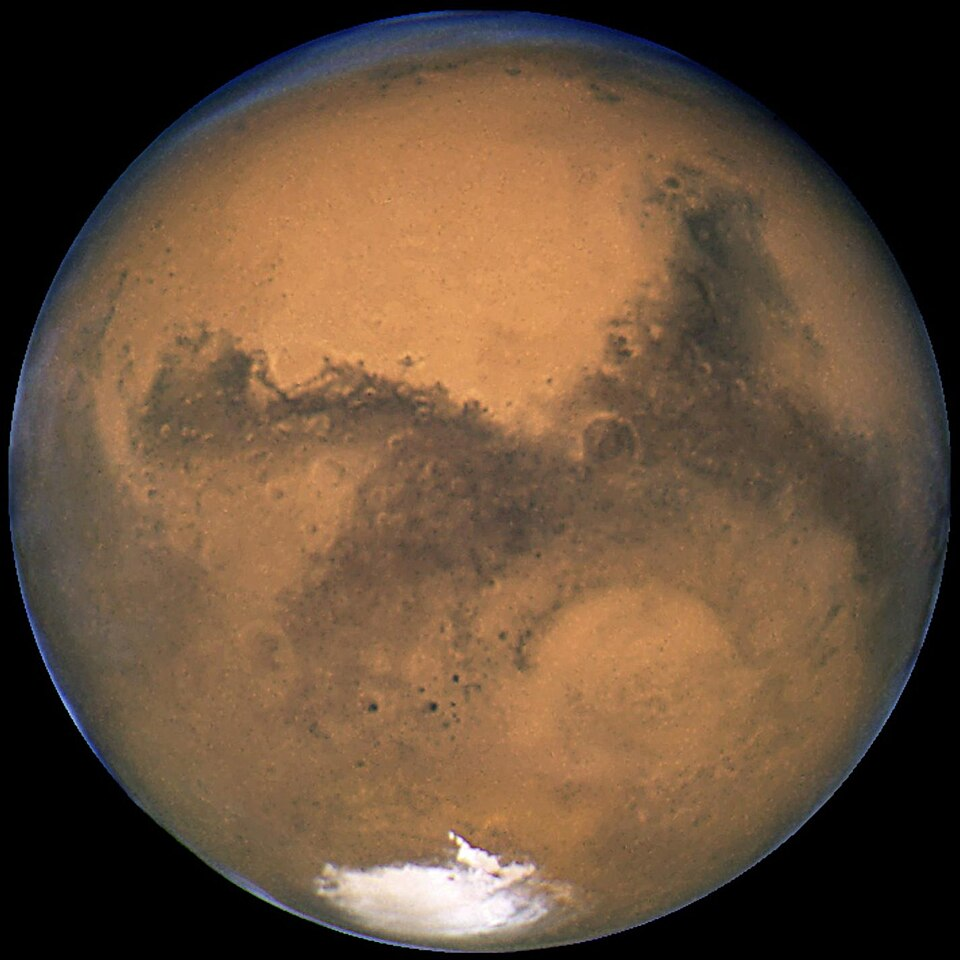
\includegraphics[width=\linewidth]{images/book1/g6-mars-hubble.jpg}\\[2pt]
{\small Mars}
\end{minipage}

\medskip
{\small Trois cartes postales de l'espace. Vénus, photographiée par la
sonde Mariner~10 en 1974~: nous ne voyons que le sommet de ses \omterm{def:g4:clouds-rain-snow:cloud}{nuages}. La
Terre, photographiée par l'équipage d'Apollo~17 en route vers la Lune en
1972~: l'Afrique, l'Arabie et la glace de l'Antarctique sous des \omterm{def:g4:clouds-rain-snow:cloud}{nuages}
blancs. Mars, photographiée par le télescope spatial Hubble en 2003, avec
une calotte blanche de glace à son \omterm{def:g3:continents-and-oceans:poles}{pôle}. (Photos~: NASA/JPL-Caltech~;
NASA~; NASA, ESA and the Hubble Heritage Team.)}
% ledger: nasa:venus-mariner10, nasa:apollo17-earth, hubble:mars-2003
\end{omfigure}

\begin{recall}
Les livres de physique ont montré que le Soleil est une étoile, une énorme
boule de gaz chaud qui brille par elle-même, et qu'une planète est un gros
corps rond qui tourne autour d'une étoile et ne brille pas par
elle-même~: nous la voyons parce qu'elle renvoie la lumière de son étoile.
Le Soleil et tout ce qui tourne autour de lui forment le Système solaire.
Chaque planète parcourt autour du Soleil un chemin appelé son orbite, et
tourne sur elle-même autour d'un axe. L'air qui nous entoure presse sur
tout ce qu'il touche~: c'est la pression de l'air. La masse volumique d'un
matériau indique combien pèse un volume donné de ce matériau~: un
centimètre cube d'eau pèse 1~gramme, donc sa masse volumique est de
1~gramme par centimètre cube~; un matériau de masse volumique plus grande
que l'eau y coule, un matériau de masse volumique plus petite y flotte.
Enfin, environ sept dixièmes de la surface de la Terre sont couverts par
l'\omterm{def:g2:water-on-earth:ocean}{océan} (\cref{ch:g2:water-on-earth}).
\end{recall}

\section{Huit planètes autour du Soleil}

Huit planètes tournent autour du Soleil. Dans l'ordre, de la plus proche à
la plus lointaine, ce sont Mercure, Vénus, la Terre, Mars, Jupiter,
Saturne, Uranus et Neptune. Une phrase peut aider à retenir cet ordre~:
\emph{Me Voici Toute Mignonne, Je Suis Une Nébuleuse} (Mercure, Vénus,
Terre, Mars, Jupiter, Saturne, Uranus, Neptune).

Le dessin ci-dessous montre les huit planètes \omterm{def:g1:landscapes-around-us:water}{côte} à \omterm{def:g1:landscapes-around-us:water}{côte}, dessinées à la
même échelle~: si une planète est deux fois plus large qu'une autre, son
cercle est lui aussi deux fois plus large.

\begin{omfigure}
\pgfplotstableread{figdata/out/grade-6-planets-sizes.dat}\gsixsizes
\begin{tikzpicture}
  \draw[black!40] (-0.2,0) -- (13.8,0);
  \pgfplotstablegetrowsof{\gsixsizes}
  \pgfmathtruncatemacro{\gsixlast}{\pgfplotsretval-1}
  \foreach \i in {0,...,\gsixlast}{
    \pgfplotstablegetelem{\i}{x_cm}\of\gsixsizes \let\gx\pgfplotsretval
    \pgfplotstablegetelem{\i}{d_cm}\of\gsixsizes \let\gd\pgfplotsretval
    \def\gn{\ifcase\i Mercure\or Vénus\or Terre\or Mars\or Jupiter\or Saturne\or Uranus\or Neptune\fi}
    \pgfplotstablegetelem{\i}{d_km}\of\gsixsizes \let\gk\pgfplotsretval
    \pgfmathsetmacro{\gr}{\gd/2}
    \ifnum\i<4
      \fill[brown!70!black, draw=black!60, line width=0.3pt] (\gx,\gr) circle (\gr);
    \else
      \fill[orange!35, draw=black!60, line width=0.3pt] (\gx,\gr) circle (\gr);
    \fi
    \node[font=\scriptsize, rotate=40, anchor=north east, inner sep=1pt]
      at (\gx+0.08,-0.08) {\gn};
  }
  \node[font=\scriptsize, align=left, anchor=north west] at (-0.2,4.15)
    {\tikz\fill[brown!70!black, draw=black!60] (0,0) circle (2.2pt); planètes rocheuses\\
     \tikz\fill[orange!35, draw=black!60] (0,0) circle (2.2pt); planètes géantes};
  \draw[|-|, black!70] (0,2.2) -- (1,2.2)
    node[midway, above, font=\scriptsize] {35\,000 km};
\end{tikzpicture}

{\small Les huit planètes dessinées à l'échelle (diamètres tirés de la fiche
de données planétaires de la NASA). Les distances qui les séparent ne sont
pas à l'échelle~: elles sont bien trop grandes pour tenir sur une page.}
% ledger: planet:Mercury.diameter, planet:Venus.diameter, planet:Earth.diameter, planet:Mars.diameter, planet:Jupiter.diameter, planet:Saturn.diameter, planet:Uranus.diameter, planet:Neptune.diameter (figdata/grade-6/planets.py, part sizes)
\end{omfigure}

Les quatre planètes les plus proches du Soleil sont petites. Les quatre
suivantes sont des géantes~: Jupiter est environ 11 fois plus large que la
Terre. Et le Soleil~? Dessiné à la même échelle que les planètes ci-dessus,
ce serait un disque d'environ 40~centimètres de diamètre --- plus large
que cette page.
% ledger: planet:Jupiter.diameter, planet:Earth.diameter, sun:R (planets.py: sun_cm = 39.9 cm)

La taille n'est pas la seule différence. Le tableau ci-dessous donne, pour
chaque planète, son diamètre, sa masse volumique (en grammes par centimètre
cube) et sa distance au Soleil.

\begin{center}
\small
\begin{tabular}{lrrrr}
\hline
planète & diamètre (km) & masse volumique (g/cm$^3$) & distance au Soleil (millions de km)\\
\hline
Mercure & 4\,879 & 5.4 & 58\\
Vénus & 12\,104 & 5.2 & 108\\
Terre & 12\,756 & 5.5 & 150\\
Mars & 6\,792 & 3.9 & 228\\
\hline
Jupiter & 142\,984 & 1.3 & 779\\
Saturne & 120\,536 & 0.7 & 1\,432\\
Uranus & 51\,118 & 1.3 & 2\,867\\
Neptune & 49\,528 & 1.6 & 4\,515\\
\hline
\end{tabular}
% ledger: planet:Mercury.diameter, planet:Venus.diameter, planet:Earth.diameter, planet:Mars.diameter, planet:Jupiter.diameter, planet:Saturn.diameter, planet:Uranus.diameter, planet:Neptune.diameter, planet:Mercury.density, planet:Venus.density, planet:Earth.density, planet:Mars.density, planet:Jupiter.density, planet:Saturn.density, planet:Uranus.density, planet:Neptune.density, planet:Mercury.dist, planet:Venus.dist, planet:Earth.dist, planet:Mars.dist, planet:Jupiter.dist, planet:Saturn.dist, planet:Uranus.dist, planet:Neptune.dist (figdata/grade-6/planets.py, main table)
\end{center}

Les masses volumiques partagent les planètes en deux familles, sans rien
entre les deux~: les quatre premières sont denses, plus de 3.9~grammes par
centimètre cube, comme la \omterm{def:g3:stones-pebbles-sand:rock}{roche} et le métal~; les quatre dernières sont
légères, moins de 1.7~gramme par centimètre cube.

\begin{definition}[Planètes rocheuses et planètes géantes]\label{def:g6:earth-a-planet:planet-types}
Une \emph{planète rocheuse}\index{planete rocheuse@planète rocheuse} est
une petite planète dense, faite de \omterm{def:g3:stones-pebbles-sand:rock}{roche} et de métal, avec une surface
solide sur laquelle une sonde peut se poser~: Mercure, Vénus, la Terre et
Mars. Une \emph{planète géante}\index{planete geante@planète géante} est une
très grosse planète de faible masse volumique, faite surtout de gaz et de
liquides, sans surface solide où se poser~: Jupiter, Saturne, Uranus et
Neptune.
% ledger: nasa:planet-families
\end{definition}

\begin{omfigure}
\begin{minipage}[c]{0.6\linewidth}\centering
\begin{tikzpicture}
  \begin{axis}[ybar, bar width=11pt, width=\linewidth, height=5.4cm,
      ymin=0, ymax=6.2, xmin=-0.6, xmax=7.6,
      xtick={0,...,7}, xticklabels={Mercure,Vénus,Terre,Mars,Jupiter,Saturne,Uranus,Neptune},
      xticklabel style={rotate=40, anchor=north east, font=\scriptsize},
      ytick={0,1,...,6}, ylabel={masse volumique (g/cm$^3$)},
      tick label style={font=\scriptsize}, label style={font=\scriptsize},
      axis x line*=bottom, axis y line*=left]
    \addplot[fill=brown!70!black, draw=black!60, bar shift=0pt, restrict x to domain=0:3]
      table[x=idx, y=density_gcm3] {figdata/out/grade-6-planets-density.dat};
    \addplot[fill=orange!35, draw=black!60, bar shift=0pt, restrict x to domain=4:7]
      table[x=idx, y=density_gcm3] {figdata/out/grade-6-planets-density.dat};
    \draw[blue!60!black, densely dashed] (axis cs:-0.6,1) -- (axis cs:7.6,1);
    \node[font=\scriptsize, blue!60!black, anchor=south, inner sep=1pt]
      at (axis cs:5,1) {eau};
  \end{axis}
\end{tikzpicture}
\end{minipage}\hfill
\begin{minipage}[c]{0.36\linewidth}\centering
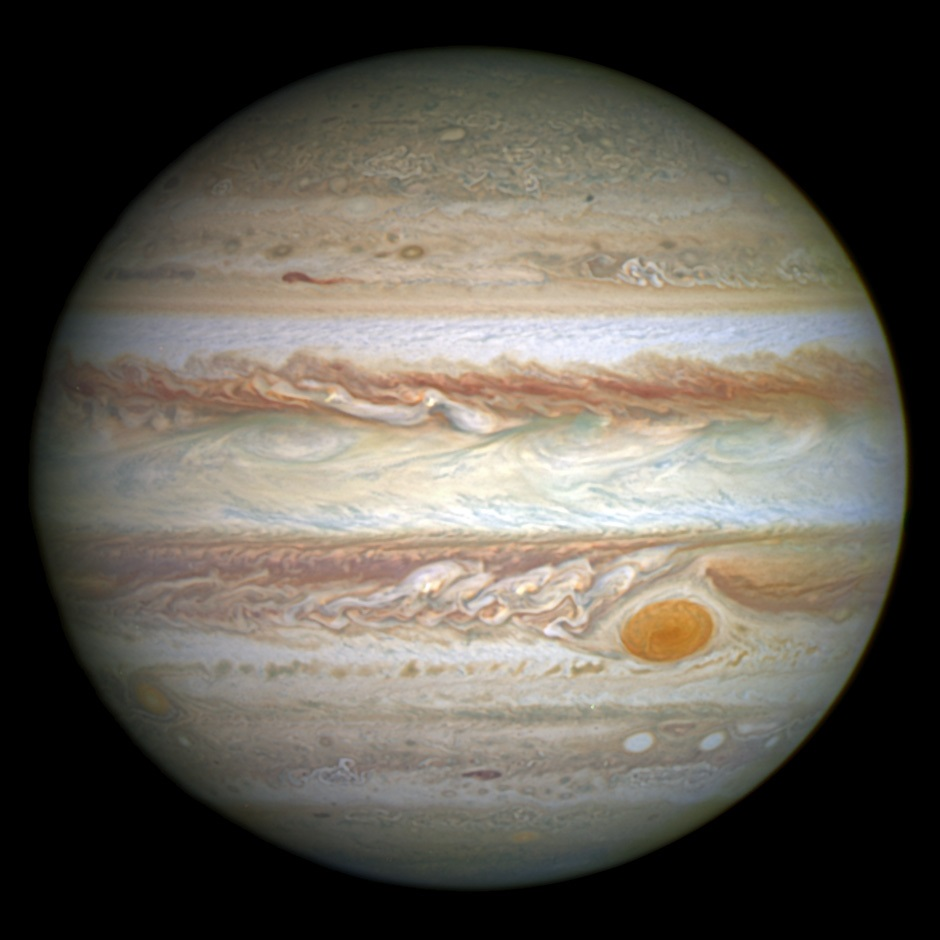
\includegraphics[width=0.9\linewidth]{images/book1/g6-jupiter-hubble.jpg}\\[2pt]
{\small Jupiter, photographiée par le télescope spatial Hubble en 2014.
(Photo~: NASA, ESA, A.~Simon.)}
% ledger: hubble:jupiter-2014
\end{minipage}

\smallskip
{\small À gauche~: la masse volumique des huit planètes~; la ligne en
tirets est celle de l'eau. À droite~: ce que nous voyons d'une \omterm{def:g6:earth-a-planet:planet-types}{planète
géante}, c'est le sommet de ses \omterm{def:g4:clouds-rain-snow:cloud}{nuages}.}
% ledger: planet:Mercury.density, planet:Venus.density, planet:Earth.density, planet:Mars.density, planet:Jupiter.density, planet:Saturn.density, planet:Uranus.density, planet:Neptune.density (figdata/grade-6/planets.py, part density)
\end{omfigure}

La photographie de Jupiter montre des bandes de \omterm{def:g4:clouds-rain-snow:cloud}{nuages}, claires et sombres,
et un ovale rouge~: la Grande Tache rouge, une \omterm{def:g5:natural-hazards:storm}{tempête} géante plus grande
que la Terre entière, qui souffle depuis des centaines d'années. Sous les
\omterm{def:g4:clouds-rain-snow:cloud}{nuages}, il n'y a pas de sol~: seulement des gaz, surtout de l'hydrogène et
de l'hélium, de plus en plus denses à mesure que l'on descend.
% ledger: nasa:jupiter-gas

\begin{remark}[Une planète plus légère que l'eau]\label{rem:g6:earth-a-planet:saturn}
Saturne est la seule planète dont la masse volumique est plus petite que
celle de l'eau~: environ 0.7~gramme par centimètre cube. S'il existait une
baignoire assez grande pour la contenir, Saturne flotterait~!
% ledger: nasa:saturn-float, planet:Saturn.density
\end{remark}

\section{À quelle distance les planètes sont-elles les unes des autres~?}

Les planètes ne sont pas seulement très différentes par leur taille~; elles
sont aussi très éloignées les unes des autres. La Terre est à environ
150~millions de kilomètres du Soleil. Neptune, la planète la plus
lointaine, est 30~fois plus loin~: à environ 4500~millions de kilomètres.
Le dessin ci-dessous place les huit planètes sur une même ligne, à leur
distance du Soleil, à l'échelle.
% ledger: planet:Earth.dist, planet:Neptune.dist

\begin{omfigure}
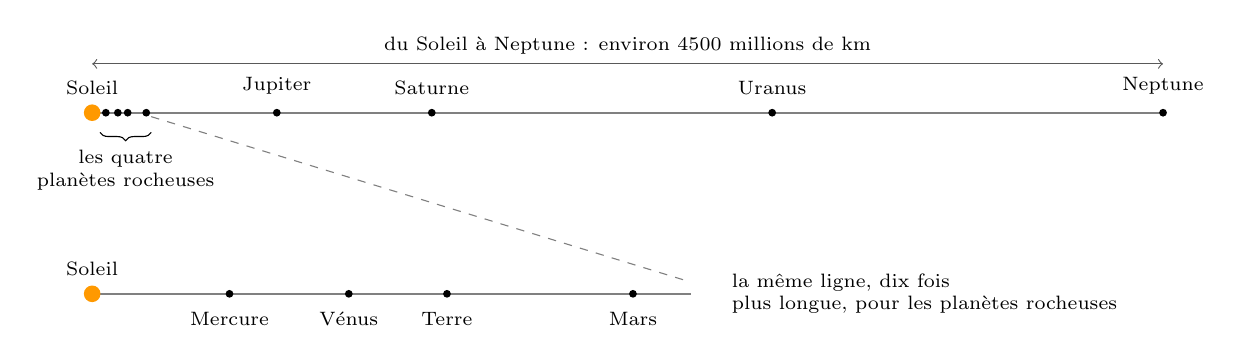
\begin{tikzpicture}
  % whole system
  \draw[thick, gray] (0,0) -- (13.6,0);
  \fill[orange!80!yellow] (0,0) circle (3pt);
  \node[font=\scriptsize, above=3pt] at (0,0) {Soleil};
  \foreach \n/\x/\lab in {Mercure/0.174/, Vénus/0.326/, Terre/0.451/, Mars/0.687/,
                          Jupiter/2.345/Jupiter, Saturne/4.313/Saturne, Uranus/8.636/Uranus, Neptune/13.6/Neptune} {
    \fill (\x,0) circle (1.4pt);
    \node[font=\scriptsize, above=3pt] at (\x,0) {\lab};
  }
  \draw[decorate, decoration={brace, amplitude=3pt, mirror}] (0.1,-0.25) -- (0.75,-0.25)
    node[midway, below=3pt, font=\scriptsize, align=center] {les quatre\\ planètes rocheuses};
  \draw[<->, thin, gray!70!black] (0,0.62) -- (13.6,0.62) node[midway, above, font=\scriptsize, black] {du Soleil à Neptune~: environ 4500 millions de km};
  % the inner system, ten times larger
  \begin{scope}[yshift=-2.3cm]
    \draw[thick, gray] (0,0) -- (7.6,0);
    \fill[orange!80!yellow] (0,0) circle (3pt);
    \node[font=\scriptsize, above=3pt] at (0,0) {Soleil};
    \foreach \n/\x in {Mercure/1.744, Vénus/3.259, Terre/4.506, Mars/6.868} {
      \fill (\x,0) circle (1.4pt);
      \node[font=\scriptsize, below=3pt] at (\x,0) {\n};
    }
    \node[font=\scriptsize, anchor=west, align=left] at (8.0,0) {la même ligne, dix fois\\ plus longue, pour les planètes rocheuses};
  \end{scope}
  \draw[dashed, gray] (0.75,-0.05) -- (7.6,-2.15);
\end{tikzpicture}

{\small Les distances des planètes au Soleil, à l'échelle. En haut~: tout le
Système solaire, du Soleil à Neptune. En bas~: les quatre \omterm{def:g6:earth-a-planet:planet-types}{planètes
rocheuses}, agrandies dix fois. La taille des points n'est pas à l'échelle.}
% ledger: planet:Mercury.dist, planet:Venus.dist, planet:Earth.dist, planet:Mars.dist, planet:Jupiter.dist, planet:Saturn.dist, planet:Uranus.dist, planet:Neptune.dist (figdata/grade-6/planets.py, part dist)
\end{omfigure}

Les quatre \omterm{def:g6:earth-a-planet:planet-types}{planètes rocheuses} sont toutes proches du Soleil~; les quatre
\omterm{def:g6:earth-a-planet:planet-types}{planètes géantes} sont loin, séparées par d'immenses intervalles. L'écart
entre Mars et Jupiter, à lui seul, environ 550~millions de kilomètres, est
plus de deux fois plus grand que la distance du Soleil à Mars.
% ledger: planet:Mars.dist, planet:Jupiter.dist

Il est difficile de dessiner les tailles et les distances à la même
échelle~: les planètes deviennent des points invisibles. Une
\emph{maquette à l'\omterm{def:g2:drawing-to-map:scale}{échelle}} aide à imaginer les deux à la fois.

\begin{method}[Construire une maquette du Système solaire à l'échelle]\label{met:g6:earth-a-planet:scale-model}
\begin{enumerate}
  \item Choisis la taille de la Terre dans la maquette, par exemple 1~cm.
  \item Cherche combien de kilomètres réels représente 1~cm de la
        maquette~: divise le diamètre réel de la Terre (12\,756~km) par sa
        taille dans la maquette.
  \item Divise chaque taille réelle et chaque distance réelle par ce
        nombre. Change ensuite d'unité pour obtenir quelque chose de facile
        à imaginer (centimètres, mètres, kilomètres).
\end{enumerate}
% ledger: planet:Earth.diameter
\end{method}

\begin{example}[Une bille pour la Terre]\label{ex:g6:earth-a-planet:marble}
Si la Terre est une bille de 1~cm de large, 1~cm représente 12\,756~km. Le
Soleil, de 1\,391\,400~km de diamètre, devient une boule de $1\,391\,400 \div 12\,756 \approx
109$~cm de large~: une boule plus haute
qu'un jeune enfant. La Terre est à 150~millions de~km du Soleil~:
$149\,600\,000 \div 12\,756 \approx 11\,700$~cm, soit environ 117~mètres,
la longueur d'un terrain de football.
% ledger: planet:Earth.diameter, sun:R, planet:Earth.dist
\end{example}

\begin{center}\small
\begin{tabular}{|l|c|c|}
\hline
\textbf{corps} & \textbf{taille dans la maquette (cm)} & \textbf{distance au Soleil (m)} \\
\hline
le Soleil & 109 & --- \\
Mercure & 0.38 & 45 \\
Vénus & 0.95 & 85 \\
la Terre & 1.00 & 117 \\
Mars & 0.53 & 179 \\
Jupiter & 11.21 & 610 \\
Saturne & 9.45 & 1123 \\
Uranus & 4.01 & 2248 \\
Neptune & 3.88 & 3540 \\
\hline
\end{tabular}
\end{center}
% ledger: sun:R, planet:Mercury.diameter, planet:Venus.diameter, planet:Earth.diameter, planet:Mars.diameter, planet:Jupiter.diameter, planet:Saturn.diameter, planet:Uranus.diameter, planet:Neptune.diameter, planet:Mercury.dist, planet:Venus.dist, planet:Earth.dist, planet:Mars.dist, planet:Jupiter.dist, planet:Saturn.dist, planet:Uranus.dist, planet:Neptune.dist (figdata/grade-6/planets.py, part model)

Dans cette maquette, tout le Système solaire jusqu'à Neptune s'étale sur un
cercle de 7~km de diamètre, avec une grosse boule au milieu, et huit billes
et boules, la plus grosse de la taille d'un pamplemousse, dispersées
autour. Le Système solaire est surtout fait de vide.

\section{Vénus, la Terre et Mars}

Vénus, la Terre et Mars sont voisines, toutes trois des \omterm{def:g6:earth-a-planet:planet-types}{planètes rocheuses}.
Vénus a presque la même taille que la Terre~: son diamètre vaut 95~\% de
celui de la Terre. Mars est plus petite~: son diamètre vaut environ la
moitié de celui de la Terre. Pourtant, ces trois planètes ne pourraient
guère être plus différentes.
% ledger: planet:Venus.diameter, planet:Earth.diameter, planet:Mars.diameter (planets.py: 94.9 %)

\paragraph{Vénus.} Vénus est enveloppée d'une épaisse couche d'air, faite
surtout de dioxyde de carbone, avec des \omterm{def:g4:clouds-rain-snow:cloud}{nuages} denses d'acide sulfurique,
un acide brûlant. Son air est si épais qu'il presse sur le sol 92~fois plus
fort que l'air de la Terre sur le nôtre. À la surface, la température est
d'environ 464~$^\circ$C~: assez pour faire fondre le plomb. Aucune eau ne
peut y rester liquide.
% ledger: nasa:venus-clouds, planet:Venus.psurf, planet:Venus.Tmean

\paragraph{Mars.} Mars est un \omterm{def:g5:weather-and-climate:desert}{désert} froid, sec et poussiéreux. Son air est
lui aussi fait surtout de dioxyde de carbone, mais il est très ténu~: il
presse sur le sol environ cent fois moins que l'air de la Terre. La
température moyenne est de $-65$~$^\circ$C. On y trouve de l'eau
aujourd'hui, mais gelée~: sous forme de glace dans les calottes polaires et
sous le sol près des \omterm{def:g3:continents-and-oceans:poles}{pôles}. Pourtant, Mars n'a pas toujours été ainsi~: il
y a des milliards d'années, des \omterm{def:g1:landscapes-around-us:water}{rivières} coulaient sur Mars, des \omterm{def:g1:landscapes-around-us:water}{lacs} se
formaient et des \omterm{def:g5:water-shapes-the-land:flood}{crues} la balayaient.
% ledger: nasa:mars-water, planet:Mars.psurf, planet:Mars.Tmean

\paragraph{La Terre.} Entre les deux, la Terre a un air qui presse sur le
sol avec environ 1~bar (l'unité utilisée pour comparer la pression de
l'air sur les planètes), une température moyenne de 15~$^\circ$C et des
\omterm{def:g2:water-on-earth:ocean}{océans} d'eau liquide.
% ledger: planet:Earth.psurf, planet:Earth.Tmean

\begin{omfigure}
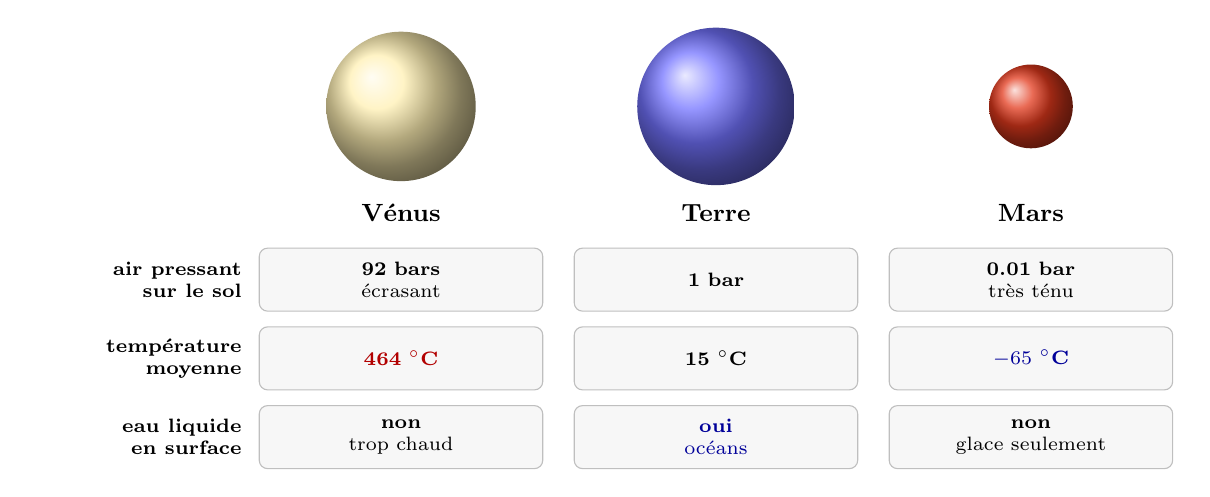
\begin{tikzpicture}[x=1cm, y=1cm,
    lab/.style={font=\scriptsize, align=center, text width=3.6cm},
    row/.style={font=\scriptsize\bfseries, anchor=east, align=right, text width=2.6cm}]
  % discs to scale: diameters 94.9 %, 100 %, 53.2 % of the Earth's (planets.py)
  \shade[ball color=yellow!60!orange!30] (3,0) circle (0.949);
  \shade[ball color=blue!55] (7,0) circle (1.0);
  \shade[ball color=red!55!brown] (11,0) circle (0.532);
  \node[font=\small\bfseries] at (3,-1.35) {Vénus};
  \node[font=\small\bfseries] at (7,-1.35) {Terre};
  \node[font=\small\bfseries] at (11,-1.35) {Mars};
  \foreach \y/\t in {-2.2/{air pressant\\sur le sol}, -3.2/{température\\moyenne},
                     -4.2/{eau liquide\\en surface}}
    {\node[row] at (1.1,\y) {\t};}
  \foreach \x in {3,7,11}{
    \foreach \y in {-2.2,-3.2,-4.2}{
      \draw[rounded corners=3pt, black!25, fill=black!3] (\x-1.8,\y-0.4) rectangle (\x+1.8,\y+0.4);}}
  \node[lab] at (3,-2.2) {\textbf{92 bars}\\écrasant};
  \node[lab] at (7,-2.2) {\textbf{1 bar}};
  \node[lab] at (11,-2.2) {\textbf{0.01 bar}\\très ténu};
  \node[lab, text=red!70!black] at (3,-3.2) {\textbf{464~$^\circ$C}};
  \node[lab] at (7,-3.2) {\textbf{15~$^\circ$C}};
  \node[lab, text=blue!60!black] at (11,-3.2) {\textbf{$-65$~$^\circ$C}};
  \node[lab] at (3,-4.2) {\textbf{non}\\trop chaud};
  \node[lab, text=blue!60!black] at (7,-4.2) {\textbf{oui}\\océans};
  \node[lab] at (11,-4.2) {\textbf{non}\\glace seulement};
\end{tikzpicture}

{\small Vénus, la Terre et Mars comparées. Les trois disques sont dessinés
à l'échelle. (Valeurs~: fiche de données planétaires de la NASA.)}
% ledger: planet:Venus.psurf, planet:Earth.psurf, planet:Mars.psurf, planet:Mercury.Tmean, planet:Venus.Tmean, planet:Earth.Tmean, planet:Mars.Tmean, planet:Jupiter.Tmean, planet:Saturn.Tmean, planet:Uranus.Tmean, planet:Neptune.Tmean, nasa:mars-water
\end{omfigure}

\paragraph{Chaud et froid.} Près du Soleil, une planète reçoit beaucoup de
sa lumière et de sa chaleur~; loin de lui, très peu. Donc plus une planète
est loin du Soleil, plus elle devrait être froide. Le diagramme ci-dessous
montre que c'est vrai à partir de la Terre et au-delà~: les \omterm{def:g6:earth-a-planet:planet-types}{planètes
géantes}, lointaines, sont des mondes gelés. Mais regarde Vénus~: elle est
presque deux fois plus loin du Soleil que Mercure, et pourtant elle est
plus chaude~! Son épais air de dioxyde de carbone retient la chaleur du
Soleil comme une lourde couverture et ne la laisse pas s'échapper. Mercure,
presque sans air, ne peut pas garder sa chaleur.
% ledger: planet:Mercury.Tmean, planet:Venus.Tmean, planet:Earth.Tmean, planet:Mars.Tmean, planet:Jupiter.Tmean, planet:Saturn.Tmean, planet:Uranus.Tmean, planet:Neptune.Tmean, planet:Mercury.dist, planet:Venus.dist, planet:Earth.dist, planet:Mars.dist, planet:Jupiter.dist, planet:Saturn.dist, planet:Uranus.dist, planet:Neptune.dist, nasa:venus-clouds, planet:Mercury.psurf

\begin{omfigure}
\begin{tikzpicture}
  \begin{axis}[ybar, bar width=14pt, width=0.86\linewidth, height=6cm,
      ymin=-270, ymax=520, xmin=-0.6, xmax=7.6,
      xtick={0,...,7},
      xticklabels={{Mercure\\58}, {Vénus\\108}, {Terre\\150}, {Mars\\228},
                   {Jupiter\\779}, {Saturne\\1432}, {Uranus\\2867}, {Neptune\\4515}},
      xticklabel style={align=center, font=\scriptsize},
      axis x line*=bottom, axis y line*=left,
      xticklabel pos=lower, ytick={-200,-100,...,500},
      ylabel={température moyenne ($^\circ$C)}, xlabel={planète et distance au Soleil (millions de km)},
      tick label style={font=\scriptsize}, label style={font=\scriptsize},
      nodes near coords, nodes near coords style={font=\tiny},
      every node near coord/.append style={/pgf/number format/1000 sep={}}]
    \addplot[fill=orange!50, draw=black!60, bar shift=0pt]
      table[x=idx, y=tmean_C] {figdata/out/grade-6-planets-temp.dat};
    \draw[black!50] (axis cs:-0.6,0) -- (axis cs:7.6,0);
  \end{axis}
\end{tikzpicture}

{\small La température moyenne des planètes, dans l'ordre de leur distance
au Soleil. Vénus fait exception~: elle est plus chaude que Mercure, qui est
plus proche du Soleil. (Valeurs~: fiche de données planétaires de la
NASA.)}
% ledger: planet:Mercury.Tmean, planet:Venus.Tmean, planet:Earth.Tmean, planet:Mars.Tmean, planet:Jupiter.Tmean, planet:Saturn.Tmean, planet:Uranus.Tmean, planet:Neptune.Tmean, planet:Mercury.dist, planet:Venus.dist, planet:Earth.dist, planet:Mars.dist, planet:Jupiter.dist, planet:Saturn.dist, planet:Uranus.dist, planet:Neptune.dist (figdata/grade-6/planets.py, part temp)
\end{omfigure}

\section{Ce qui rend la vie possible sur la Terre}

La Terre est la seule planète où nous savons que la vie existe. Les êtres
vivants ont besoin de plusieurs conditions réunies, et la Terre les a
toutes.

\begin{itemize}
  \item \textbf{De l'eau liquide.} Tous les êtres vivants ont besoin d'eau
        liquide~: la Terre a des \omterm{def:g2:water-on-earth:ocean}{océans}, des \omterm{def:g1:landscapes-around-us:water}{rivières} et des \omterm{def:g1:landscapes-around-us:water}{lacs}.
  \item \textbf{Des températures douces.} À la surface de la Terre, l'eau
        gèle à 0~$^\circ$C et bout à 100~$^\circ$C (physique). Avec une
        moyenne de 15~$^\circ$C, les températures de la Terre restent
        surtout entre les deux, et son eau reste donc liquide.
  \item \textbf{La bonne distance au Soleil.} Plus près du Soleil, comme
        Vénus, une planète risque de devenir trop chaude~; plus loin, comme
        Mars, trop froide. La Terre est à la bonne distance pour avoir de
        l'eau liquide.
  \item \textbf{Une atmosphère.} La couche d'air qui entoure la Terre garde
        sa surface chaude la nuit, donne aux êtres vivants les gaz dont ils
        ont besoin, et presse assez sur les \omterm{def:g2:water-on-earth:ocean}{océans} pour que leur eau reste
        liquide. Sur Mars, l'air est si ténu que l'eau liquide ne peut pas
        durer longtemps en surface~: elle gèle ou se transforme en vapeur.
\end{itemize}
% ledger: nasa:mars-water, planet:Earth.Tmean

\begin{remark}[Y a-t-il eu de la vie sur Mars~?]\label{rem:g6:earth-a-planet:mars-life}
Puisque Mars a eu autrefois des \omterm{def:g1:landscapes-around-us:water}{rivières} et des \omterm{def:g1:landscapes-around-us:water}{lacs}, les scientifiques se
demandent si de minuscules êtres vivants ont pu y vivre, il y a très
longtemps, quand Mars était plus chaude et humide. Les scientifiques ne
s'attendent pas à trouver des êtres vivants sur Mars aujourd'hui~; avec
des robots mobiles, ils cherchent dans ses \omterm{def:g3:stones-pebbles-sand:rock}{roches} des traces d'une vie qui
aurait existé il y a très longtemps.
% ledger: nasa:mars-water
\end{remark}

\section{La Terre vue de l'espace}

Pendant des milliers d'années, les hommes n'ont pu qu'imaginer à quoi leur
planète ressemblait vue de l'extérieur. Le 24~décembre~1968, les
astronautes d'Apollo~8, en orbite autour de la Lune, ont vu la Terre se
lever au-dessus de l'horizon gris de la Lune, et l'un d'eux, Bill Anders,
a pris la photographie ci-dessous.
% ledger: nasa:earthrise

\begin{omfigure}
\begin{minipage}[c]{0.46\linewidth}\centering
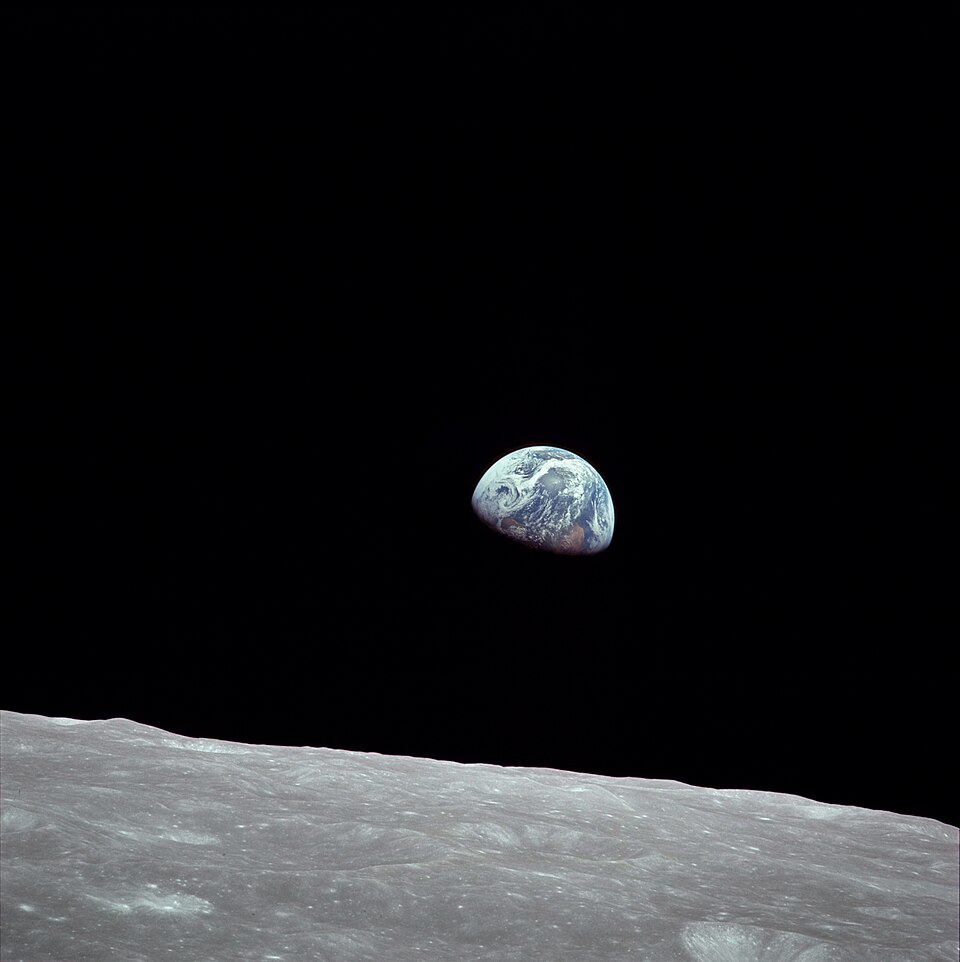
\includegraphics[width=0.85\linewidth]{images/book1/g6-earthrise.jpg}
\end{minipage}\hfill
\begin{minipage}[c]{0.5\linewidth}
{\small \emph{Lever de Terre}~: la Terre au-dessus de l'horizon de la Lune,
photographiée depuis Apollo~8 en orbite autour de la Lune, le
24~décembre~1968. (Photo~: NASA, Bill Anders.)}

\medskip
{\small Regarde les couleurs~: le bleu des \omterm{def:g2:water-on-earth:ocean}{océans}, les tourbillons blancs
des \omterm{def:g4:clouds-rain-snow:cloud}{nuages}, le brun des terres. Tout autour, le noir de l'espace~; au
premier plan, le sol gris et mort de la Lune, sans eau et sans air.}
\end{minipage}
% ledger: nasa:earthrise
\end{omfigure}

Vue de l'espace, la Terre est surtout bleue~: l'\omterm{def:g2:water-on-earth:ocean}{océan} couvre environ sept
dixièmes de sa surface. Des \omterm{def:g4:clouds-rain-snow:cloud}{nuages} blancs de gouttelettes d'eau
tourbillonnent au-dessus, et de la glace blanche couvre les \omterm{def:g3:continents-and-oceans:poles}{pôles}. Les
terres sont brunes là où elles sont sèches, vertes là où poussent des
plantes. L'air lui-même est invisible, mais les \omterm{def:g4:clouds-rain-snow:cloud}{nuages} qui y flottent
montrent qu'il est là. De toutes les planètes du Système solaire, seule la
Terre montre ces couleurs réunies~: de l'eau liquide, des \omterm{def:g4:clouds-rain-snow:cloud}{nuages} et des
plantes vivantes.
% ledger: wss:ocean-cover, nasa:apollo17-earth

\begin{history}[Le point bleu pâle]
\begin{minipage}[c]{0.66\linewidth}
Le 14~février~1990, la sonde spatiale Voyager~1 se trouvait à environ
6~milliards de kilomètres du Soleil, plus loin que Neptune. Avant de
laisser le Système solaire derrière elle, elle a tourné sa caméra et pris
une image de la Terre. Sur la photographie, notre planète n'est qu'un seul
point brillant, plus petit qu'un grain de poussière, pris dans un rayon de
soleil. L'astronome Carl Sagan a écrit à son sujet~: «~Regardez encore ce
point. C'est ici. C'est chez nous. C'est nous.~»
% ledger: nasa:pale-blue-dot
\end{minipage}\hfill
\begin{minipage}[c]{0.3\linewidth}\centering
\begin{tikzpicture}
  \node[inner sep=0] (img) {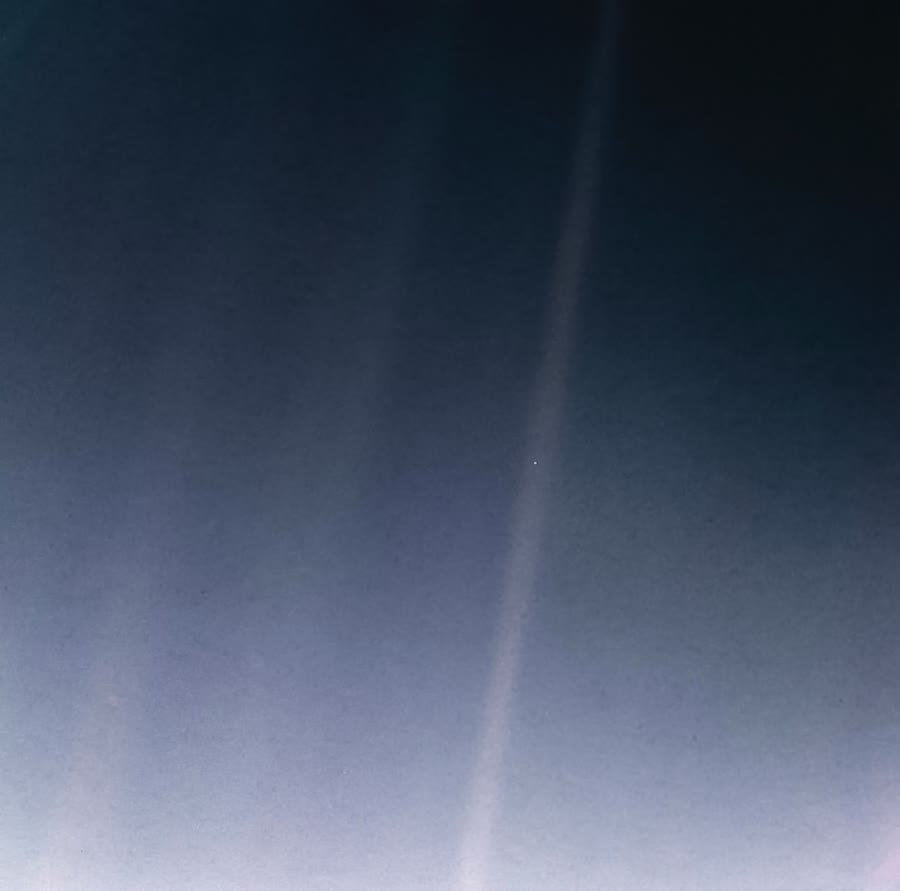
\includegraphics[width=\linewidth]{images/book1/g6-pale-blue-dot.jpg}};
  \draw[yellow!80!orange, thick] ($(img.south west)!0.594!(img.south east) + (0,{0.476*\linewidth})$) circle (6pt);
\end{tikzpicture}\\[2pt]
{\footnotesize La Terre (entourée) vue par Voyager~1, 1990. (Image~:
NASA/JPL-Caltech, domaine public.)}
% ledger: nasa:pale-blue-dot
\end{minipage}
\end{history}

\section{Exercices}

\begin{exercise}[$\star$]\label{exo:g6:earth-a-planet:1}
Range les huit planètes du Système solaire dans l'ordre, de la plus proche
du Soleil à la plus lointaine. Souligne les \omterm{def:g6:earth-a-planet:planet-types}{planètes rocheuses}.
\end{exercise}

\begin{exercise}[$\star$]\label{exo:g6:earth-a-planet:2}
Recopie et complète~: «~Une \omterm{def:g6:earth-a-planet:planet-types}{planète rocheuse} est petite et \ldots, avec
une \ldots{} solide. Une \omterm{def:g6:earth-a-planet:planet-types}{planète géante} est très grande, de faible \ldots,
faite surtout de \ldots{} et de \ldots{}~»
\end{exercise}

\begin{exercise}[$\star$]\label{exo:g6:earth-a-planet:3}
D'après le tableau de ce chapitre, quelle planète a le diamètre le plus
proche de celui de la Terre~? Quelle est la plus grande planète~? La plus
petite~?
\end{exercise}

\begin{exercise}[$\star$]\label{exo:g6:earth-a-planet:4}
Vrai ou faux~? Corrige les phrases fausses.
(a) Vénus est couverte d'\omterm{def:g2:water-on-earth:ocean}{océans}.
(b) Mars est plus froide que la Terre.
(c) Les \omterm{def:g6:earth-a-planet:planet-types}{planètes géantes} sont les quatre planètes les plus proches du Soleil.
(d) Saturne est moins dense que l'eau.
\end{exercise}

\begin{exercise}[$\star\star$]\label{exo:g6:earth-a-planet:5}
Le diamètre de Mercure est de 4\,879~km, celui de la Terre de
12\,756~km. Calcule le diamètre de Mercure en pourcentage de celui de la
Terre, arrondi à l'unité.
% ledger: planet:Mercury.diameter, planet:Earth.diameter (planets.py: 38.2 %)
\end{exercise}

\begin{exercise}[$\star\star$]\label{exo:g6:earth-a-planet:6}
Combien de Terres, \omterm{def:g1:landscapes-around-us:water}{côte} à \omterm{def:g1:landscapes-around-us:water}{côte}, tiendraient sur le diamètre de Saturne
(120\,536~km)~? Arrondis à l'unité. Saturne est-elle une \omterm{def:g6:earth-a-planet:planet-types}{planète rocheuse}
ou une \omterm{def:g6:earth-a-planet:planet-types}{planète géante}~?
% ledger: planet:Saturn.diameter, planet:Earth.diameter
\end{exercise}

\begin{exercise}[$\star\star$]\label{exo:g6:earth-a-planet:7}
Les astronomes ont découvert des planètes autour d'autres étoiles. La
planète~A a une masse volumique de 1.1~gramme par centimètre cube et elle
est 9~fois plus large que la Terre. La planète~B a une masse volumique de
5.0~grammes par centimètre cube et elle est un peu plus petite que la
Terre. Laquelle est une \omterm{def:g6:earth-a-planet:planet-types}{planète rocheuse}, et laquelle une \omterm{def:g6:earth-a-planet:planet-types}{planète
géante}~? Explique.
\end{exercise}

\begin{exercise}[$\star\star$]\label{exo:g6:earth-a-planet:8}
D'après le diagramme des températures des planètes~: (a) de combien de
degrés Vénus est-elle plus chaude que la Terre~? (b) De combien de degrés
Mars est-elle plus froide que la Terre~?
% ledger: planet:Venus.Tmean, planet:Earth.Tmean, planet:Mars.Tmean
\end{exercise}

\begin{exercise}[$\star\star$]\label{exo:g6:earth-a-planet:9}
Mercure est la planète la plus proche du Soleil, mais Vénus est la plus
chaude. Explique pourquoi.
\end{exercise}

\begin{exercise}[$\star\star$]\label{exo:g6:earth-a-planet:10}
La Terre est à 150~millions de kilomètres du Soleil et Mars à
228~millions de kilomètres. De combien de millions de kilomètres Mars
est-elle plus loin du Soleil~? De quel pourcentage la distance de Mars
est-elle plus grande que celle de la Terre (arrondis à l'unité)~?
% ledger: planet:Earth.dist, planet:Mars.dist
\end{exercise}

\begin{exercise}[$\star\star\star$]\label{exo:g6:earth-a-planet:11}
Un ami dit~: «~Mars a toujours été un \omterm{def:g5:weather-and-climate:desert}{désert} sec~; il n'y a jamais eu d'eau
là-bas.~» À l'aide de ce chapitre, réponds-lui~: qu'avait Mars il y a des
milliards d'années, où est son eau aujourd'hui, et pourquoi l'eau liquide
ne peut-elle pas durer à sa surface maintenant~?
\end{exercise}

\begin{exercise}[$\star\star\star$]\label{exo:g6:earth-a-planet:12}
On dit parfois que Vénus est la jumelle de la Terre. Son diamètre vaut
95~\% de celui de la Terre, et l'attraction de la pesanteur à sa surface
vaut 8.9 sur une échelle où celle de la Terre vaut 9.8. (a) Calcule
l'attraction de la pesanteur de Vénus en pourcentage de celle de la Terre,
arrondie à l'unité. (b) Donne deux points sur lesquels Vénus ressemble à
une jumelle de la Terre, et deux points sur lesquels elle ne lui ressemble
pas.
% ledger: planet:Venus.gravity, planet:Earth.gravity, planet:Venus.diameter
\end{exercise}

\section{Problème~: Cartes postales de trois planètes}

\begin{problem}[{Problème du week-end --- trois cartes postales de l'espace, et la force
avec laquelle l'air de Vénus presse sur son sol}]
\label{pb:g6:earth-a-planet:1}
% ledger: planet:Venus.dist, planet:Venus.diameter, planet:Venus.density, planet:Venus.Tmean, planet:Venus.psurf, planet:Earth.dist, planet:Earth.diameter, planet:Earth.density, planet:Earth.Tmean, planet:Earth.psurf, planet:Mars.dist, planet:Mars.diameter, planet:Mars.density, planet:Mars.Tmean, planet:Mars.psurf, nasa:venus-clouds, nasa:mars-water
Trois sondes robotisées envoient chacune une carte postale, avec quelques
nombres écrits au dos.

\begin{center}
\small
\begin{tabular}{>{\raggedright\arraybackslash}p{0.29\linewidth}>{\raggedright\arraybackslash}p{0.29\linewidth}>{\raggedright\arraybackslash}p{0.29\linewidth}}
\hline
\textbf{De Vénus} & \textbf{De la Terre} & \textbf{De Mars}\\
\hline
Distance au Soleil~: 108~millions de~km. & Distance au Soleil~:
150~millions de~km. & Distance au Soleil~: 228~millions de~km.\\
Diamètre~: 12\,104~km. & Diamètre~: 12\,756~km. & Diamètre~: 6\,792~km.\\
Masse volumique~: 5.2~g/cm$^3$. & Masse volumique~: 5.5~g/cm$^3$. & Masse volumique~: 3.9~g/cm$^3$.\\
Température moyenne~: 464~$^\circ$C. & Température moyenne~: 15~$^\circ$C. &
Température moyenne~: $-65$~$^\circ$C.\\
L'air presse sur le sol avec 92~bars. D'épais \omterm{def:g4:clouds-rain-snow:cloud}{nuages} d'acide. &
L'air presse sur le sol avec 1~bar. Des \omterm{def:g2:water-on-earth:ocean}{océans} et des \omterm{def:g4:clouds-rain-snow:cloud}{nuages}. &
L'air presse sur le sol avec 0.01~bar. De la glace aux \omterm{def:g3:continents-and-oceans:poles}{pôles}.\\
\hline
\end{tabular}
\end{center}

\medskip
\noindent\textbf{Partie I --- Les planètes comparées.}
\begin{enumerate}
  \item Range les trois planètes dans l'ordre de leur distance au Soleil.
  \item De combien de millions de kilomètres Vénus est-elle plus proche du
        Soleil que la Terre~? De combien de millions de kilomètres Mars
        est-elle plus loin~?
  \item Calcule le diamètre de Mars en pourcentage de celui de la Terre,
        arrondi à l'unité. Mars fait-elle environ le quart, la moitié ou les
        trois quarts de la largeur de la Terre~?
  \item Ces trois planètes sont-elles des \omterm{def:g6:earth-a-planet:planet-types}{planètes rocheuses} ou des
        \omterm{def:g6:earth-a-planet:planet-types}{planètes géantes}~? Quels nombres des cartes postales te
        l'indiquent~?
\end{enumerate}

\medskip
\noindent\textbf{Partie II --- L'air.}
\begin{enumerate}[resume]
  \item Sur quelle planète l'air est-il le plus épais~? Sur laquelle est-il
        le plus ténu~?
  \item Combien de fois moins l'air de Mars presse-t-il sur son sol que
        l'air de la Terre sur le nôtre~?
  \item Vénus est plus proche du Soleil que la Terre, mais cela seul
        n'explique pas une température de 464~$^\circ$C. Que fait l'air de
        Vénus à la chaleur du Soleil~?
  \item Combien de fois plus fort que sur la Terre l'air presse-t-il sur le
        sol de Vénus~? Pourquoi une sonde qui se pose sur Vénus doit-elle
        avoir des parois très solides~?
\end{enumerate}

\medskip
\noindent\textbf{Partie III --- L'eau et la vie.}
\begin{enumerate}[resume]
  \item À la surface de la Terre, l'eau gèle à 0~$^\circ$C et bout à
        100~$^\circ$C. À l'aide des températures moyennes, explique pourquoi
        l'eau est liquide sur la Terre.
  \item Que deviendrait un verre d'eau posé sur le sol de Vénus~? Sur le sol
        de Mars~?
  \item Mars avait des \omterm{def:g1:landscapes-around-us:water}{rivières} et des \omterm{def:g1:landscapes-around-us:water}{lacs} il y a des milliards d'années.
        Que nous apprend cela sur le \omterm{def:g5:weather-and-climate:climate}{climat} de Mars autrefois, comparé à
        celui d'aujourd'hui~?
  \item Écris le dos de la carte postale de la Terre~: en quelques phrases,
        donne quatre raisons pour lesquelles la vie est possible sur la
        Terre.
\end{enumerate}
\end{problem}
